%%%%%%%%%%%%%%%%%%% 使用Latexmk编译 %%%%%%%%%%%%%%%%%%%%%%%

\documentclass[10pt]{article}
\usepackage{ctex}
\usepackage{NotesTeXV3,lipsum}
\usepackage{graphicx}
%\usepackage{showframe}
\begin{document}
    \title{通信电子线路}
	\author{}
	\maketitle
	\newpage
%    \pagestyle{fancynotes}
    \part{绪论}
    \section{非线性电子线路的作用}
    利用器件的非线性完成振荡、频率变换等功能的电路统称为非线性电子线路。
    非线性电子线路分为3类:功率放大器、振荡器、调制解调器

    \par
   电磁波的传播方式:
   \begin{enumerate}
    \item 沿地表 \quad $1.5MHZ$ \quad $\lambda > 200m$
    \item 电离层反射 \quad $1.5MHZ ~ 30MHZ$ \quad $10 m <\lambda < 200m$\quad (传播距离、时间最长)
    \item 沿直线传播波 \quad $30MHZ$以上 \quad $\lambda < 10m $
   \end{enumerate} 

   \par
   无线通信系统由发射装置、接收装置和传输媒质组成。\\
   发射装置包括:换能器、发射机、发射天线。
   \begin{figure}[H] %H为当前位置,!htb为忽略美学标准,htbp为浮动图形
    \centering %图片居中
    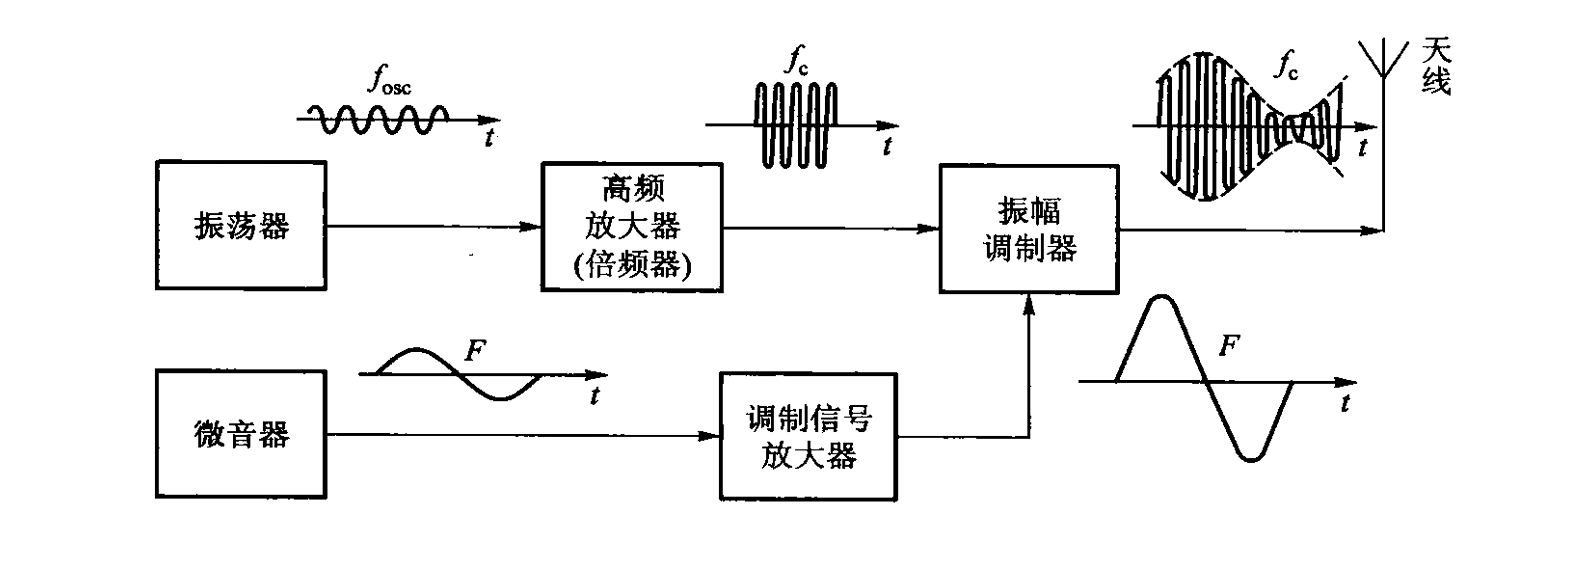
\includegraphics[width=0.7\textwidth]{pictures/1-1.png} %插入图片,[]中设置图片大小,{}中是图片文件名
    \caption{采用调幅方式的发射机组成框图} %最终文档中希望显示的图片标题
    \label{fig.1-1} %用于文内引用的标签
    \end{figure}
    \marginnote{调制型号放大器(又称低频放大器),由多级放大器组成,前面几级为小信号放大器,后面几级为功率放大器}
   接收装置包括:接收天线、接收机、换能器
   \begin{figure}[H] %H为当前位置,!htb为忽略美学标准,htbp为浮动图形
    \centering %图片居中              
    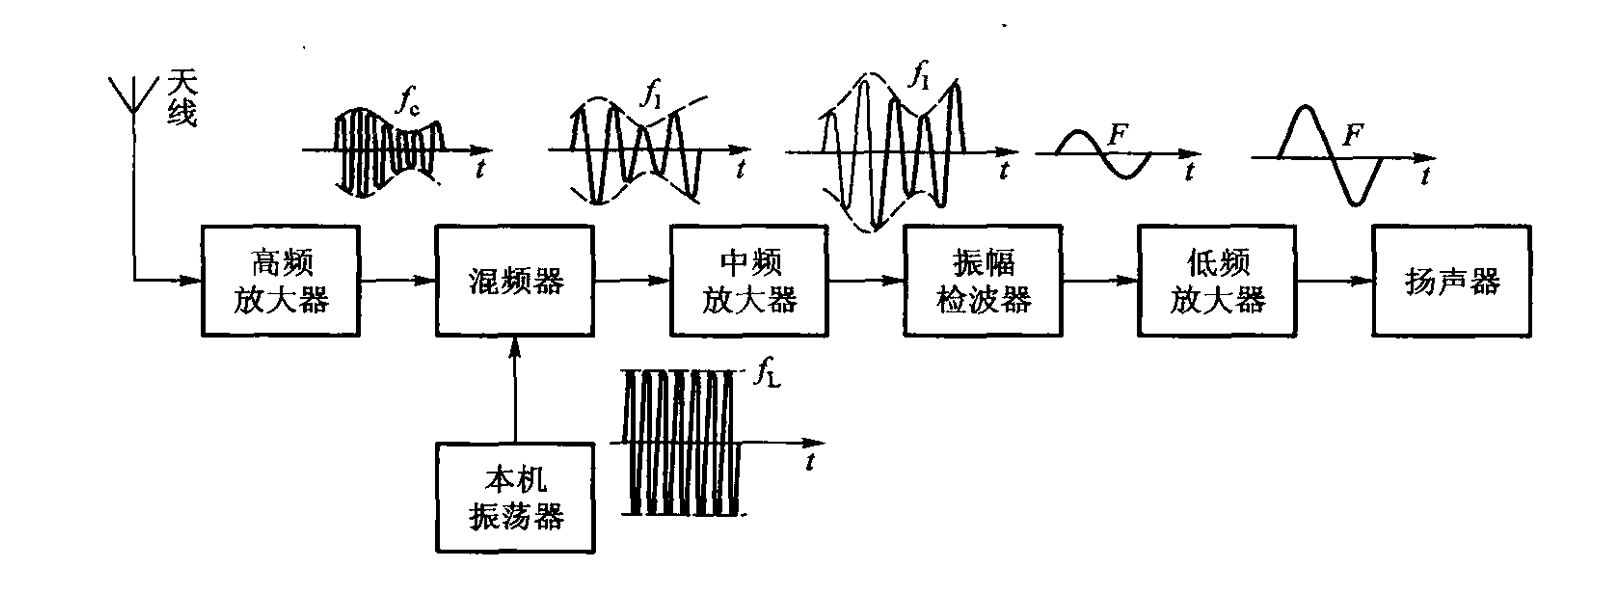
\includegraphics[width=0.7\textwidth]{pictures/1-2.png} %插入图片,[]中设置图片大小,{}中是图片文件名
    \caption{采用调幅方式的接收机组成框图(超外差式)} %最终文档中希望显示的图片标题
    \label{fig.1-1} %用于文内引用的标签
    \end{figure}
    \marginnote{混频器可以提高解调能力,$f_I = |f_L - f_c|$ 为一固定数值}
    调制有调辐、调频、调相三种,调频和调相统称为调角。携带有信息的电信号称为调制信号,未调制的高频振荡信号称为载波信号。
    经过调制后的高频振荡信号称为已调波信号。\par
    解调是调制的逆过程,将已调波信号变换为携带信息的电信号。\par
    只有信号波长与天线尺寸可以比拟的时候,天线才能有效辐射和接收电磁波,调制可以显著减小天线尺寸。
    调制可以电信号载到不同频率的载波信号上,接收机就可以根据频率选出信息,抑制其他信息干扰。
\section{非线性器件的基本特点}
    直流电导:\par
    $$
    g_0 |_Q = \frac{I_Q}{V_Q}
    $$
    交流电导/增量电导/微变电导:\par
    $$
    g|_Q = \frac{di}{dv}
    $$
    平均电导:基波电流振幅与外加电压振幅的比值
    $$
    g_{av}|_{Q,V_m} = \frac{I_{1m}}{V_m}
    $$

   \begin{figure}[H] %H为当前位置,!htb为忽略美学标准,htbp为浮动图形
    \centering %图片居中
    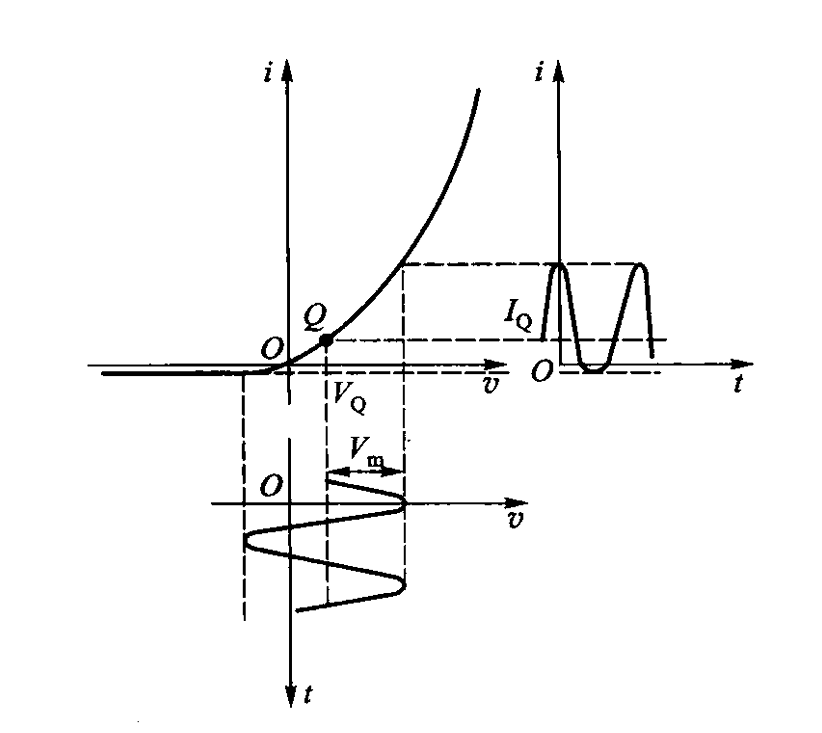
\includegraphics[width=0.7\textwidth]{pictures/1-3.png} %插入图片,[]中设置图片大小,{}中是图片文件名
    \caption{$g_{av}$定义} %最终文档中希望显示的图片标题
    \label{fig.1-1} %用于文内引用的标签
    \end{figure}

 非线性器件不满足叠加定理

\newpage
\part{功率电子线路}
\section{功率电子线路概述}
\subsection{功率放大器}
功率放大器的要求:安全、高效、不失真地输出所需信号功率\par
功率放大器是能量转化器,直流电源提供直流功率$P_D$,一部分转化为输出信号功率$P_o$,其余部分小号在集电极。
集电极效率$\eta_C$,定义为:
$$
\eta_C = \frac{P_o}{P_D} = \frac{P_o}{P_o + P_C}
$$

功率管的应用状态:
\begin{table}[h]
    \centering
    \begin{tabular}{|c|c|c|c|c|}
    \hline
    类型 & 甲类 & 乙类 & 甲乙类&丙类 \\
    \hline
    导通时间 & 一个周期 & 半个周期 &甲类和乙类之间& 小于半个周期 \\
    \hline
    \end{tabular}
    \caption{各种状态下的导通时间}
    \label{tab:example}
\end{table}

\begin{figure}[H] %H为当前位置,!htb为忽略美学标准,htbp为浮动图形
 \centering %图片居中
 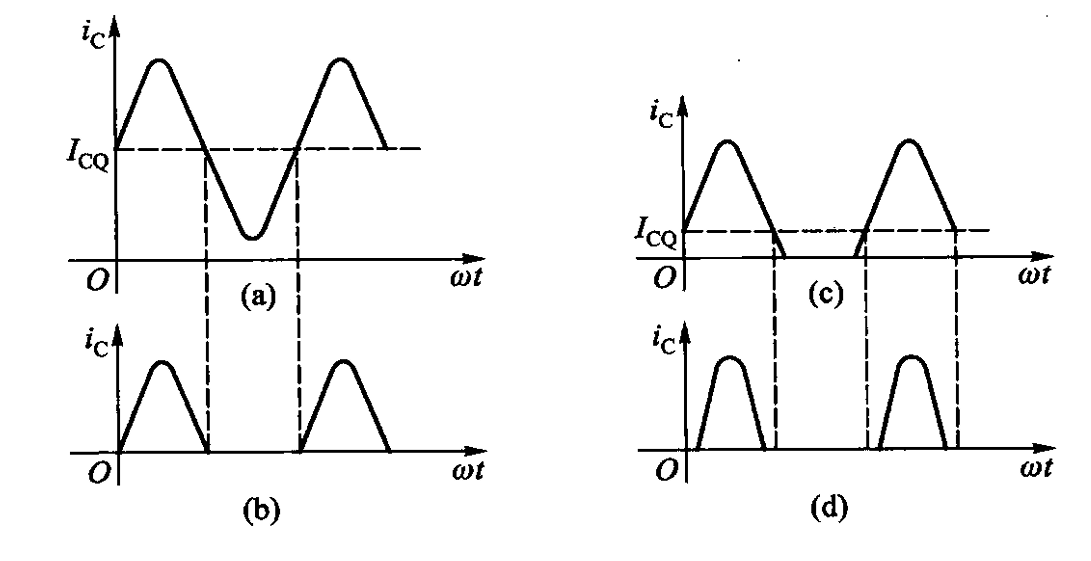
\includegraphics[width=0.7\textwidth]{pictures/2-1.png} %插入图片,[]中设置图片大小,{}中是图片文件名
 \caption{(a)甲类\quad(b)乙类\quad(c)甲乙类\quad(d)丙类 } %最终文档中希望显示的图片标题
 \label{fig.1-1} %用于文内引用的标签
 \end{figure}

 集电极耗散功率$P_C$:
 \begin{equation}
   P_C = \frac{1}{2\pi} \int_{0}^{2\pi} i_Cv_{CE} \, dt
\end{equation}
减小管子在一个周期内的导通时间可增大效率,$\eta_C$丙类$>$乙类$>$甲类,该效率的运用状态都是波形严重失真。、
\par
\subsection{电源变换电路}
\normalsize
\begin{enumerate}
    \item 整流器:交流变直流
    \item 直流-直流变换器
    \item 逆变器:直流变交流
    \item 交流-交流变换器
\end{enumerate}
\subsection{功率器件}
功率器件:散热、$P_{CM}$、二次击穿要看一下
\section{功率放大器的电路组成和工作特性}
功率管为大信号工作,性能分析时必须用大信号模型。工程上多用图解分析法。
\begin{example}
    以基本放大器为例,分析功率性能。
\begin{figure}[H] %H为当前位置,!htb为忽略美学标准,htbp为浮动图形
 \centering %图片居中
 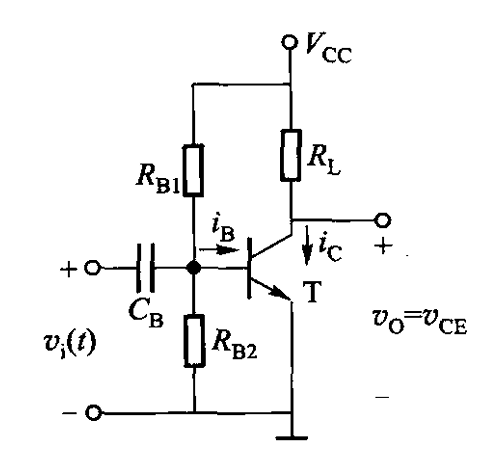
\includegraphics[width=0.4\textwidth]{pictures/2-2.png} %插入图片,[]中设置图片大小,{}中是图片文件名
 \caption{基本放大器} %最终文档中希望显示的图片标题
 \label{fig.1-1} %用于文内引用的标签
 \end{figure}
假设忽略$V_{CE(on)}$和$I_{CEO}$,
设工作点$V_{CEQ} = \frac{V_{CC}}{2}$,$I_{CQ} = \frac{V_{CEQ}}{R_L} = \frac{V_{CC}}{2R_L}$ 
在最大幅值的情况下($v_{im} = \frac{V_{CC}}{2}$)
\begin{align*}
    i_C &= I_{CQ} + I_{cm}\sin(\omega t) \\
    v_{CE} &= V_{CEQ} - v_{cm}\sin(\omega t)
\end{align*}
直流功率$P_D$,负载功率$P_o$,集电极功率$P_C$,分别为
\begin{align}
P_D = \frac{1}{2\pi}\int_{0}^{2\pi}V_{CC}i_{C}dt = V_{CC}I_{CQ}\\
P_L = \frac{1}{2\pi}\int_{0}^{2\pi}i_{C}^2R_L d\omega t  = V_{CEQ}I_{CQ}+\frac{1}{2}V_{cm}I_{cm}\\
P_C =  \frac{1}{2\pi}\int_{0}^{2\pi} v_{CE}i_{C} = V_{CEQ}I_{C}-\frac{1}{2}V_{cm}I_{cm}
\end{align}
\end{example}

\marginnote{$P_o$是负载的得到的信号功率,$P_L$是负载得到的所有功率,有交流和直流两部分,
只有交流部分(信号功率$P_o$)是希望得到的}
$P_D$只于电源电压和工作点有关,$P_L$ 和 $P_C$都由交流和直流两部分组成,且表达式相同,只是$P_L$是加交流功率,$P_C$是减。
$P_L$的交流项为$P_o = \frac{P_D}{4}$,只有这一部分是希望输出的。如果不加信号,管子的负载功率和集电极功率相同,加上信号后,
集电极减少的功率即为负载所得的信号功率。\par
基本放大器的集电极最大功率
$$
\eta_{Cmax} = \frac{P_o}{P_D} = \frac{1}{4} = 25\%
$$
如果考虑$V_{CE(sat)}$和$I_{CEO}$,该效率会更低,另外,功率管的集电极饱和压降$V_{CE(sat)}$会大于$0.3V$
\newpage
\part{谐振功率放大器}
\section{谐振功率放大器工作原理}

\end{document}